\begin{figure}[h!]
	\centering
	
	
	
	\tikzset{every picture/.style={line width=0.75pt}} %set default line width to 0.75pt        
	
	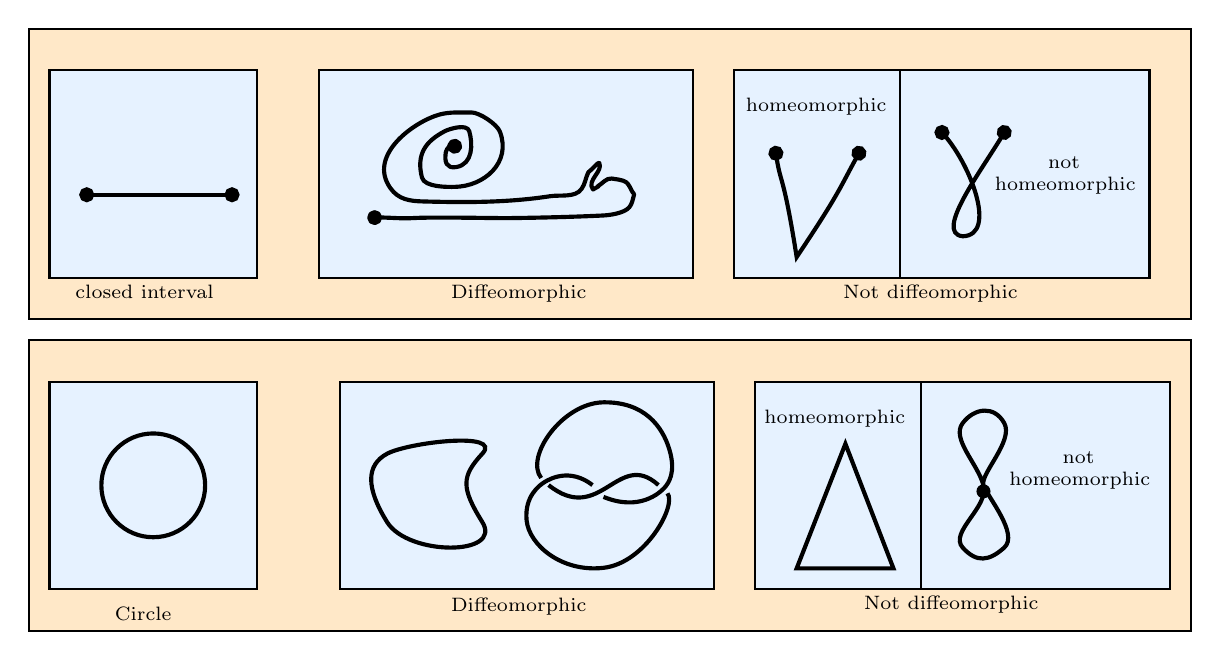
\begin{tikzpicture}[x=0.75pt,y=0.75pt,yscale=-1,xscale=1]
		%uncomment if require: \path (0,300); %set diagram left start at 0, and has height of 300
		
		%Shape: Rectangle [id:dp5759997839543596] 
		\draw  [fill={rgb, 255:red, 255; green, 232; blue, 200 }  ,fill opacity=1 ] (40,157) -- (600,157) -- (600,297) -- (40,297) -- cycle ;
		%Shape: Rectangle [id:dp09502642053448573] 
		\draw  [fill={rgb, 255:red, 255; green, 232; blue, 200 }  ,fill opacity=1 ] (40,7) -- (600,7) -- (600,147) -- (40,147) -- cycle ;
		%Shape: Rectangle [id:dp794045496594401] 
		\draw  [fill={rgb, 255:red, 230; green, 242; blue, 255 }  ,fill opacity=1 ] (50,27) -- (150,27) -- (150,127) -- (50,127) -- cycle ;
		%Straight Lines [id:da6087895159341825] 
		\draw [line width=1.5]    (67.96,87) -- (110,87) -- (137.96,87) ;
		\draw [shift={(137.96,87)}, rotate = 0] [color={rgb, 255:red, 0; green, 0; blue, 0 }  ][fill={rgb, 255:red, 0; green, 0; blue, 0 }  ][line width=1.5]      (0, 0) circle [x radius= 2.61, y radius= 2.61]   ;
		\draw [shift={(67.96,87)}, rotate = 0] [color={rgb, 255:red, 0; green, 0; blue, 0 }  ][fill={rgb, 255:red, 0; green, 0; blue, 0 }  ][line width=1.5]      (0, 0) circle [x radius= 2.61, y radius= 2.61]   ;
		%Shape: Rectangle [id:dp09862432189325276] 
		\draw  [fill={rgb, 255:red, 230; green, 242; blue, 255 }  ,fill opacity=1 ] (180,27) -- (360,27) -- (360,127) -- (180,127) -- cycle ;
		%Curve Lines [id:da7044859223189306] 
		\draw [line width=1.5] [line join = round][line cap = round]   (206.67,98) .. controls (212.79,97.77) and (218.84,98.62) .. (224.95,98.25) .. controls (235.26,97.63) and (264.87,98.34) .. (271.54,98.25) .. controls (286.57,98.05) and (301.61,97.71) .. (316.62,97) .. controls (319.63,96.86) and (326.92,95.98) .. (329.4,92.99) .. controls (330.76,91.34) and (331.06,89.03) .. (331.65,86.97) .. controls (331.78,86.5) and (331.16,86.13) .. (330.9,85.71) .. controls (330.36,84.84) and (329.2,81.93) .. (327.89,80.95) .. controls (326.37,79.8) and (322.33,79.43) .. (320.88,79.19) .. controls (318.33,78.78) and (316.36,81.67) .. (314.12,82.95) .. controls (313.62,83.24) and (316.75,81.75) .. (311.86,84.46) .. controls (308.57,80.06) and (317.01,75.65) .. (314.87,71.67) .. controls (314.51,71.01) and (311.61,74.68) .. (309.61,76.18) .. controls (308.2,79.09) and (308.2,81.56) .. (306.35,84.21) .. controls (303.36,88.5) and (296.24,86.93) .. (291.08,87.72) .. controls (270.68,90.82) and (251.05,90.76) .. (230.21,90.23) .. controls (223.63,90.06) and (218.16,89.37) .. (214.18,83.71) .. controls (203.05,67.86) and (225.81,51.67) .. (237.98,48.34) .. controls (242.9,47) and (248.15,47.41) .. (253.26,47.34) .. controls (257.1,47.29) and (265.65,52.98) .. (267.03,56.62) .. controls (272.72,71.56) and (259.41,82.95) .. (245.24,83.21) .. controls (242.23,83.26) and (230.67,83.51) .. (229.46,78.69) .. controls (226.65,67.44) and (231.14,61.28) .. (240.48,56.37) .. controls (242.38,55.37) and (251.15,52.51) .. (252.25,56.37) .. controls (254,62.5) and (254.12,72.26) .. (245.99,73.67) .. controls (241.17,74.51) and (240.2,71.1) .. (240.98,66.4) .. controls (241.21,65.02) and (243.76,61.42) .. (245.24,63.64) ;
		\draw [shift={(245.24,63.64)}, rotate = 56.35] [color={rgb, 255:red, 0; green, 0; blue, 0 }  ][fill={rgb, 255:red, 0; green, 0; blue, 0 }  ][line width=1.5] [line join = round][line cap = round]     (0, 0) circle [x radius= 2.61, y radius= 2.61]   ;
		\draw [shift={(206.67,98)}, rotate = 357.79] [color={rgb, 255:red, 0; green, 0; blue, 0 }  ][fill={rgb, 255:red, 0; green, 0; blue, 0 }  ][line width=1.5] [line join = round][line cap = round]     (0, 0) circle [x radius= 2.61, y radius= 2.61]   ;
		%Shape: Rectangle [id:dp17014344801268177] 
		\draw  [fill={rgb, 255:red, 230; green, 242; blue, 255 }  ,fill opacity=1 ] (460,27) -- (580,27) -- (580,127) -- (460,127) -- cycle ;
		%Shape: Rectangle [id:dp22662056681483733] 
		\draw  [fill={rgb, 255:red, 230; green, 242; blue, 255 }  ,fill opacity=1 ] (380,27) -- (460,27) -- (460,127) -- (380,127) -- cycle ;
		%Curve Lines [id:da6145254850720514] 
		\draw [line width=1.5]    (510,57) .. controls (499.75,74.5) and (475.75,105.5) .. (490,107) .. controls (507.25,106.5) and (493.25,71) .. (480,57) ;
		\draw [shift={(480,57)}, rotate = 226.58] [color={rgb, 255:red, 0; green, 0; blue, 0 }  ][fill={rgb, 255:red, 0; green, 0; blue, 0 }  ][line width=1.5]      (0, 0) circle [x radius= 2.61, y radius= 2.61]   ;
		\draw [shift={(510,57)}, rotate = 120.36] [color={rgb, 255:red, 0; green, 0; blue, 0 }  ][fill={rgb, 255:red, 0; green, 0; blue, 0 }  ][line width=1.5]      (0, 0) circle [x radius= 2.61, y radius= 2.61]   ;
		%Shape: Rectangle [id:dp31913409751177024] 
		\draw  [fill={rgb, 255:red, 230; green, 242; blue, 255 }  ,fill opacity=1 ] (50,177) -- (150,177) -- (150,277) -- (50,277) -- cycle ;
		%Shape: Rectangle [id:dp035182155141359805] 
		\draw  [fill={rgb, 255:red, 230; green, 242; blue, 255 }  ,fill opacity=1 ] (190,177) -- (370,177) -- (370,277) -- (190,277) -- cycle ;
		%Shape: Rectangle [id:dp7290551523037767] 
		\draw  [fill={rgb, 255:red, 230; green, 242; blue, 255 }  ,fill opacity=1 ] (470,177) -- (590,177) -- (590,277) -- (470,277) -- cycle ;
		%Shape: Rectangle [id:dp9828205444947584] 
		\draw  [fill={rgb, 255:red, 230; green, 242; blue, 255 }  ,fill opacity=1 ] (390,177) -- (470,177) -- (470,277) -- (390,277) -- cycle ;
		%Shape: Circle [id:dp8999286469461747] 
		\draw  [line width=1.5]  (75,227) .. controls (75,213.19) and (86.19,202) .. (100,202) .. controls (113.81,202) and (125,213.19) .. (125,227) .. controls (125,240.81) and (113.81,252) .. (100,252) .. controls (86.19,252) and (75,240.81) .. (75,227) -- cycle ;
		%Shape: Regular Polygon [id:dp619536170202954] 
		\draw  [line width=1.5]  (212.65,211.78) .. controls (222.84,206.3) and (268.73,200.82) .. (258.53,211.78) .. controls (248.34,222.74) and (248.34,228.22) .. (258.53,244.67) .. controls (268.73,261.11) and (222.84,261.11) .. (212.65,244.67) .. controls (202.45,228.22) and (202.45,217.26) .. (212.65,211.78) -- cycle ;
		%Curve Lines [id:da7142664625345396] 
		\draw [line width=1.5]    (290.47,226.87) .. controls (315.47,246.81) and (323.94,209.21) .. (343.39,226.87) ;
		%Curve Lines [id:da5535164021641068] 
		\draw [line width=1.5]    (286.9,223.45) .. controls (278.85,213.26) and (297.22,187.28) .. (316.93,187) .. controls (336.64,186.71) and (345.37,198.67) .. (348.68,209.78) .. controls (351.99,220.89) and (348.28,226.02) .. (346.17,228.29) .. controls (344.05,230.57) and (334.26,239.69) .. (316.93,232.57) ;
		%Curve Lines [id:da772702812520371] 
		\draw [line width=1.5]    (347.76,230.86) .. controls (352.28,236.59) and (337.17,264.47) .. (316.93,266.74) .. controls (296.69,269.02) and (281.08,255.64) .. (279.89,243.96) .. controls (278.7,232.28) and (286.14,226.88) .. (288.49,225.45) .. controls (290.83,224.01) and (300.57,218.32) .. (311.64,226.87) ;
		
		%Shape: Triangle [id:dp7950611477426] 
		\draw  [line width=1.5]  (433.48,207) -- (456.62,267) -- (410,267) -- cycle ;
		%Shape: Polygon Curved [id:ds6158924144504883] 
		\draw  [line width=1.5]  (490,197) .. controls (495.75,189.5) and (505.25,188.5) .. (510,197) .. controls (514.75,205.5) and (498.18,221.64) .. (500,227) .. controls (501.82,232.36) and (517.25,250.5) .. (510,257) .. controls (502.75,263.5) and (496.75,264.5) .. (490,257) .. controls (483.25,249.5) and (502.75,237.5) .. (500,227) .. controls (497.25,216.5) and (484.25,204.5) .. (490,197) -- cycle ;
		%Shape: Circle [id:dp2069132244539451] 
		\draw  [fill={rgb, 255:red, 0; green, 0; blue, 0 }  ,fill opacity=1 ] (497.13,229.88) .. controls (497.13,228.29) and (498.41,227) .. (500,227) .. controls (501.59,227) and (502.88,228.29) .. (502.88,229.88) .. controls (502.88,231.46) and (501.59,232.75) .. (500,232.75) .. controls (498.41,232.75) and (497.13,231.46) .. (497.13,229.88) -- cycle ;
		%Curve Lines [id:da9430641490320497] 
		\draw [line width=1.5]    (400,67) .. controls (402.25,83) and (403.25,74.5) .. (410,117) .. controls (431.75,84.5) and (430.75,83.5) .. (440,67) ;
		\draw [shift={(440,67)}, rotate = 299.28] [color={rgb, 255:red, 0; green, 0; blue, 0 }  ][fill={rgb, 255:red, 0; green, 0; blue, 0 }  ][line width=1.5]      (0, 0) circle [x radius= 2.61, y radius= 2.61]   ;
		\draw [shift={(400,67)}, rotate = 82] [color={rgb, 255:red, 0; green, 0; blue, 0 }  ][fill={rgb, 255:red, 0; green, 0; blue, 0 }  ][line width=1.5]      (0, 0) circle [x radius= 2.61, y radius= 2.61]   ;
		
		% Text Node
		\draw (61,129) node [anchor=north west][inner sep=0.75pt]  [font=\scriptsize] [align=left] {closed interval};
		% Text Node
		\draw (80,284) node [anchor=north west][inner sep=0.75pt]  [font=\scriptsize] [align=left] {Circle};
		% Text Node
		\draw (242,129) node [anchor=north west][inner sep=0.75pt]  [font=\scriptsize] [align=left] {Diffeomorphic};
		% Text Node
		\draw (431,129) node [anchor=north west][inner sep=0.75pt]  [font=\scriptsize] [align=left] {Not diffeomorphic};
		% Text Node
		\draw (384,39) node [anchor=north west][inner sep=0.75pt]  [font=\scriptsize] [align=left] {homeomorphic};
		% Text Node
		\draw (504,67) node [anchor=north west][inner sep=0.75pt]  [font=\scriptsize] [align=left] {\begin{minipage}[lt]{49.95pt}\setlength\topsep{0pt}
				\begin{center}
					not\\homeomorphic
				\end{center}
				
		\end{minipage}};
		% Text Node
		\draw (242,280) node [anchor=north west][inner sep=0.75pt]  [font=\scriptsize] [align=left] {Diffeomorphic};
		% Text Node
		\draw (441,279) node [anchor=north west][inner sep=0.75pt]  [font=\scriptsize] [align=left] {Not diffeomorphic};
		% Text Node
		\draw (511,209) node [anchor=north west][inner sep=0.75pt]  [font=\scriptsize] [align=left] {\begin{minipage}[lt]{49.95pt}\setlength\topsep{0pt}
				\begin{center}
					not\\homeomorphic
				\end{center}
				
		\end{minipage}};
		% Text Node
		\draw (393,189) node [anchor=north west][inner sep=0.75pt]  [font=\scriptsize] [align=left] {homeomorphic};
		
		
	\end{tikzpicture}
\end{figure}